\section{Diskussion}
Under denna del kommer en diskussion angående om resultaten ske samt metoderna som användes.

\subsection{Resultat}
Resultaten måste anses vara rimliga. Den första frågeställningen ställer frågan om det går att implementera en kvadratiska optimeringslösare i programspråket C. Resultatet visar att det går att implementera en sådan lösare i språket C. Anledningen till att det går är för att C är ett turingkomplett språk, dvs ett språk som kan beräkna samtliga beräkningsbara problem i det, givet tillräcklig tid och tillräckligt minnesutrymme. Språket C jobbar också väldigt nära hårdvara, vilket i sin tur gör att koden som har skrivits av kandidatgruppen kan exekvera snabbare än vad den skulle göra i andra språk. Det enda kandidatgruppen saknade i språket C var att kunna överlagra operatorer. Med hjälp av att kunna överlagra operatorer skulle t.ex. matrismultiplikationer ske med ett enkelt gånger-tecken istället för att göra ett funktionsanrop. Detta skulle ha kunnat medföra enklare kod, som i sin tur kan vara lättare att underhålla. 
\newline
\newline
Den andra frågeställningen kandidatgruppen hade var om QuadOpt skulle kunna lösa kvadratiska optimeringsproblem snabbare än Gurobi. Svaret vart nej. Anledningen till detta är att Gurobi är en kommersiell programvara som har arbetats med under en väldigt lång tid av välbetalda utvecklare och konsulter. Medan QuadOpt inte har haft samma förutsättningar. Kandidatgruppen skulle förutom att skapa en optimeringsalgoritm också skapa ett GUI och en parser i Python. Dessutom skulle kandidatgruppen även delta i diverse olika entreprenörskapskurser, förbereda opponeringar och skriva en massa dokument. Det ska också tilläggas att kandidatgruppen gjorde ett eget matrisbibliotek. Detta tog upp mycket av tiden som fanns för kandidatprojektet. Om några av dessa moment inte fanns med skulle kandidatgruppen kunna lagt dessa timmar på optimeringsalgoritmen och möjligtvis kunna matcha Gurobis hastighet.
\newline
\newline
Den sista frågeställningen kandidatgruppen hade var om man kunde utföra projektet utan någon speciell utvecklingsmetodik. Denna frågeställning är nog den svåraste att ge ett konkret svar på. Kandidatgruppen svarade ja, det går att utföra ett projekt utan någon speciell utvecklingsmetodik. Däremot så anser vissa individer i kandidatgruppen att en utvecklingsmetodik alltid finns där, även om man inte vet om det. Det som vill få sagts är att oavsett hur man jobbar, så jobbar man på ett speciellt sätt och detta är en sorts utvecklingsmetodik, men inte en officiell sådan.

\subsection{Metod}
Valet av kvadratisk optimeringsalgoritm kan ses som aningen naiv. Hade kandidatgruppen dock haft mer kunskap om ämnet hade vi kunnat resonerat mer kring vilken algoritm som skulle använts och vägt för- och nackdelar mellan dessa. Huvudanledning till att valet föll för Active-set metoden är för att kandidatgruppens kontaktperson rekommenderade den, men han sa också åt kandidatgruppen att undersöka de andra algoritmerna. I efterhand tror kandidatgruppen att Interior point metoden skulle varit lättare att utföra i C-kod och dessutom lösa problemet snabbare än vad Active-set metoden gör. Visserligen vet inte kandidatgruppen vilka problem som skulle kunna uppkomma om man skulle implementera Interior point och frågan om vilket val som är rätt endast kan besvaras genom att implementera alla de tre metoderna som jämfördes i början för att sedan ta ett beslut.
\newline
\newline
Att implementera ett matrisbibliotek är något som kandidatgruppen valde att göra för att de biblioteken som fanns tillhands var alldeles för svåra att begripa. Valet av att implementera ett matrisbibliotek var inget som var planerat under förstudien och detta tog väldigt många timmar att implementera samt att testa. Kandidatgruppen är nöjda med valet av att implementera ett eget matrisbibliotek, mycket på grund av att man vet vad som finns och hur det funkar, sen kan de som tar över projektet utvidga biblioteket hur mycket de vill. \textcolor{red}{Martin kanske vill tillägga något}
\newline
\newline
Kandidatgruppen hade kontakt med kunden främst genom e-mail och träffades vid enstaka möten. Relationen mellan kandidatgruppen och kunden har varit bra och inga problem har dykt upp. Kandidatgruppen skulle möjligtvis kunnat ha visat kunden arbetet som har gjorts vid flera tillfällen. 
\newline
\newline
Valet av att gå in i iterationer utan en utvecklingsmetodik är inget kandidatgruppen ångrar. Som tidigare nämnt kan en kandidatgrupp jobba på ett visst sätt som liknar en utvecklingsmetodik utan att veta om det. I detta fall ledde ledde arbetssättet till en variant av utvecklingsmetodiken eXtreme programming.

\subsection{Arbetet i ett vidare sammanhang}
Utöver att projektet har bidragit till vår egen och Saabs nytta kan projektet ha påverkat och ha framtida påverkan på samhället och miljön vi lever i. Mycket av informationen nedanför är hämtad direkt från Saabs hemsida och kan vara vinklad.   

\subsubsection{Etiska och samhälleliga aspekter}
Att utveckla teknik åt ett företag som förser regeringar, myndigheter och företag med militära tjänster och produkter reser många etiska frågor, till exempel: 
\begin{itemize}
\item Etiskt rätt att utveckla och sälja vapen?
\item Hur kan man förhindra att vapen och känslig information hamnar i fel händer? 
\end{itemize} 
Vapen som stridsflygplanet JAS 39 Gripen kan döda många människor och orsaka kaos i världen, varför existerar det då sådana vapen? Samhällen idag (och sedan lång tid tillbaka) har ett behov av vapen för att kunna försvara sig mot varandra, terroristgrupper och enskilda individer som av någon anledning vill attackera. Utan krig och orättvisor hade efterfrågan på Gripen saknats. I en perfekt värld hade det alltså inte existerat några vapen. Tyvärr är inte världen perfekt. 
\newline
\newline
Saabs vision med sina produkter och deras etiska riktlinjer avser att människor ska kunna känna sig säkra. Dessa riktlinjer kan dock ifrågasättas av Saabs kunder (mer om detta senare). Om vapnen inte används för att döda oskyldiga utan endast för att bidra till ett säkrare samhälle kan det ses som etiskt rätt att utveckla och sälja vapen. 
\newline
\newline   
På Saabs hemsida kan man läsa att de har polisyn noll tolerans mot korruption och att det finns många åtgärder för att uppfylla detta. I figur~\ref{fig:zerotolerance} visas en grafisk överblick över deras huvudsakliga åtgärder. 
\leavevmode
\begin{figure}[h]
	\centering
	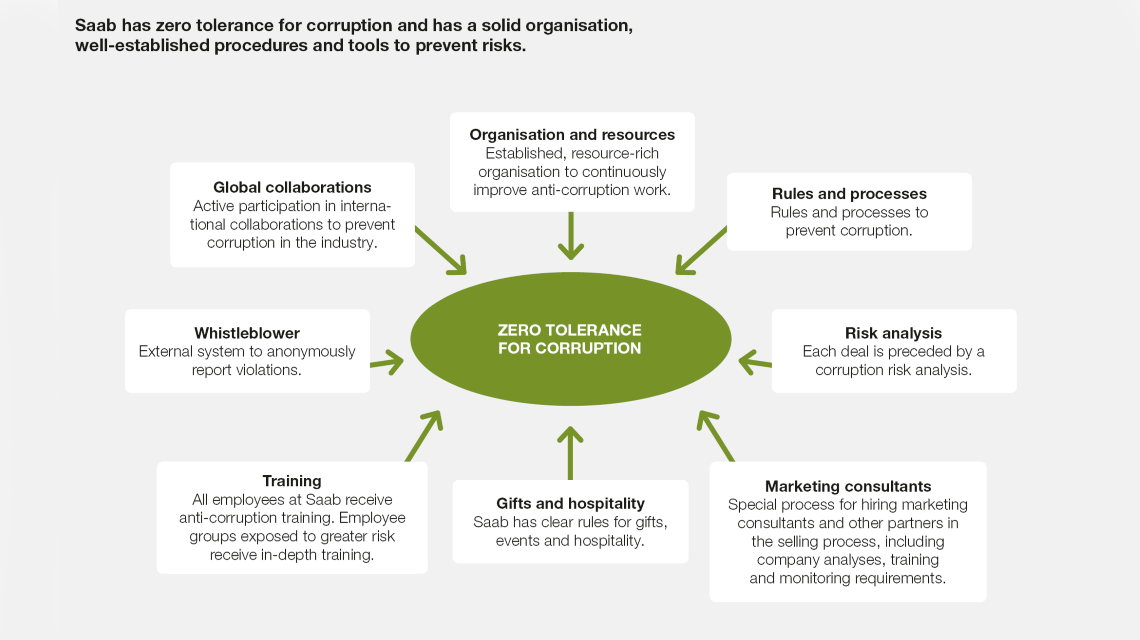
\includegraphics[scale=1.4]{grafik/modell_zero_corruption_1140x640.png}
	\caption{Zero tolerance}\label{fig:zerotolerance}
\end{figure}  
\\
Till exempel gör Saab alltid riskanalyser i samband med affärer för avgöra om det finns risk för korruption. De undersöker risker med vart affären äger rum, vem köparen är, hur upphandlingen går till och hur köparen kom i kontakt med företaget. Om riskerna inte gick att eliminera eller inte var hanterbara drar sig Saab ur affären. Detta är en åtgärd för att förhindra att produkterna hamnar i fel händer. 
\newline
\newline
När utomstående parter är inblandade och flödet av pengar inte är helt under Saabs kontroll finns det alltid risker att produkterna kan hamna i fel händer. För att minimera riskerna ser Saab till att deras etiska värden och riktlinjer strikt följs av utomstående/tillfälligt anställda konsulter och partners. Dessa partners måste genomgå utbildning och skriva under att följa Saabs etiska värden och riktlinjer. I avtalen ingår det att Saab har rätt till att kontrollera om riktlinjerna verkligen följs.   
\newline
\newline
För att förhindra korruption inom företaget utbildar Saab all personal inom ämnet. De har även ett system kallat ''Whistleblower'' för att rapportera suspekta aktiviteter och som garanterar rapporterarens anonymitet.              
\newline
\newline
Utöver vapen levererar Saab bland annat system för väderstationer, minröjning och att detektera kemiska, biologiska, radioaktiva samt kärnvapen. \citep{security}

\subsubsection{Miljöaspekter}
Vårat projekt är inte en skada för miljön eftersom det endast är samling algoritmer för att lösa och visualisera optimeringsproblem.  
\newline
\newline
Om Saab skulle använda vårat projekt i jaktflygplanet JAS 39 Gripen som projektet härstammar ifrån, uppkommer frågor kring hur pass miljövänliga företaget Saab och Gripen är. På deras hemsida \citep{saabimpact} kan man läsa om deras arbete för att minska avtrycket på miljön. De har till exempel satt upp som mål att reducera deras koldioxidutsläpp från försäljningar med tjugo procent till år 2020. I figur~\ref{fig:saabkoldioxid} visas Saabs koldioxidutsläpp och deras mål.   
\leavevmode
\begin{figure}[h]
	\centering
	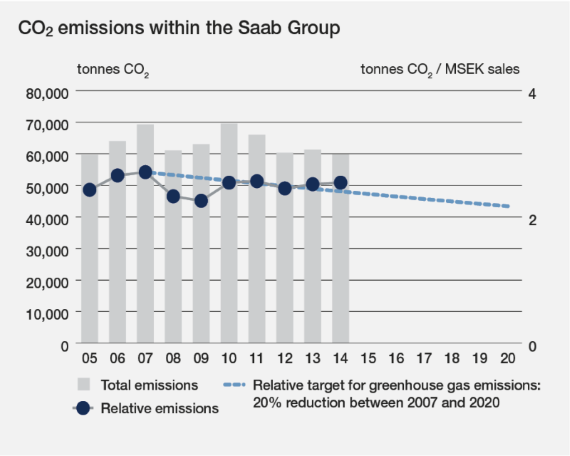
\includegraphics[scale=1.5]{grafik/saabemissions.png}
	\caption{Saabs koldioxidutsläpp}\label{fig:saabkoldioxid}	
\end{figure} 
\\
För att nå målet arbetar Saab med att reducera elförbrukningen på deras fabriker och utsläpp från resor vilka är de största faktorerna för deras koldioxidutsläpp. Genom att fokusera på att ändra de anställdas vanor, ny teknik och strategisk planering av fabrikerna har de lyckats sänka koldioxidutsläppen från fabrikerna med tjugo procent mellan åren 2009 och 2014. För att minska utsläppen från resor nämner Saab bland annat att de uppmuntrar resfria möten och samåkningar.
\newline
\newline 
Deras hantering av miljöfarliga ämnen möter EU's förordning REACH (Registration, Evaluation and Authorisation of Chemicals) som strävar efter att förbättra skyddet av människors hälsa och miljön från risker som kan förorsakas av kemikalier \citep{reach}. 
Saab är även kontributör till projektet Clean Sky som är det mest ambitiösa luftfartsforskningsprogrammet i Europa. Målet med Clean Sky är att utveckla ny teknik för att göra luftfarten mer miljövänlig med mindre bullriga och mer bränsleeffektiva flygplan. \citep{cleansky}     
\newline
\newline
Stridsflygplanet JAS 39 Gripen använder i dagsläget en jetmotor som drivs på fotogen. Fotogen är ett fossilt bränsle som leder till koldioxidutsläpp vid förbränning. Detta gör Gripen till ett system som bidrar till miljöförstöring. 
\newline
\newline
Det verkar som att Saab har ambitioner om att själva bli miljövänligare och att bidra till utvecklingen av miljövänligare teknik. De gör dock fortfarande ett negativt avtryck på miljön eftersom det sker utsläpp av koldioxid och de använder miljöfarliga ämnen i deras produkter. Detta kan dock ses som en direkt följd av att det idag tyvärr inte är lönsamt att använda eller existerar effektiv miljövänlig el och teknik.  
\newline
\newline
Skulle användandet av vårat projekt göra någon skillnad? Detta går tyvärr inte att svara på då vi saknar uppgifter på hur våran optimeringslösare skulle bidra till miljövänligheten hos stridsflygplanet JAS 39 Gripen.        